\section{$S=1$ Magnetometry}
We begin by considering a triplet state, that is a $S=1$ system.

Under the influence of a magnetic field, the Hamiltonian can be expressed as:
\begin{equation}
	H_{} = H_{\ce{D}} + H_{\ce{Z}}}
	\label{eq:nv_hamil}
\end{equation}

Here the labels $\ce{D}$ and $\ce{Z}$ describe the electron spin-spin interactions and the Zeeman interaction with an external magnetic field.

They have the following forms:
\begin{eqnarray}
	H_{\ce{D}} &=& D S_z^2 + E(S_x^2 + S_y^2) \label{H_D} \\
	H_{\ce{Z}} &=& g \mu_B \sum_{j}^{x,y,z} B_j \cdot S_j \label{H_Z} \\
\end{eqnarray}

\subsubsection{Spin-Spin Interaction}

The $E$ and $D$ in equation \ref{H_D} represent the fine structure constants of the spin
system, describing the spin-spin interaction and $S_j$ the corresponding spin operators
in x,y and z-direction.

$D$ is non-zero in system with axis of threefold (or other manifold) symmetry.
The definiteness, orientation and magnitude of $D$ is dependent on the specific spin system being studied.

$E$ occurs when there is a distortion of the point group symmetry, for example strain or an $\vec{E}$ field.
Similarly, the value of $E$ is a characteristic of the nature of the distortion and
the specifics of the spin system being studied.

\subsubsection{Zeeman Interaction}

$B_j$ in equation \ref{H_Z} is the magnetic field along the $x$, $y$ and $z$ direction, $g$ is the $g$-factor of the vacancy and $\mu_B$ the Bohr-Magneton.

% It seems often the scaled parameter $g\mu_B$ is considered, for the $\ce{NV^-}$ system this is around $28\;\ce{ GHz T^{-1}}$, but again, will be a characteristic of the system being studied. 

% \subsubsection{Reduced Hamiltonian}
By combining $H_{\ce{D}}$ and $H_{\ce{Z}}$
we find
\begin{equation}
	H_{} = D S_z^2 + E(S_x^2 + S_y^2) + g \mu_B \sum_{j}^{x,y,z} B_j \cdot S_j
	\label{eq:reduced_H_NV}
\end{equation}

the $S=1$ spin operators \eqref{eq:s1_spin_operators}, then aligning the magnetic field (with strength $B_0$) along the $z$-axis (the quantisation axis), the reduced Hamiltonian will have the form
\begin{equation}
	H_{} = \begin{pmatrix}
		D + B_0 & 0 & E     \\
		0       & 0 & 0     \\
		E       & 0 & D-B_0
	\end{pmatrix},
	\label{eq:reduced_H_NV_matrix}
\end{equation}

with Eigenvalues

\begin{equation}
	E_x = E_y = D \pm \sqrt{B_0^2  + E^2}, \; E_z = 0.
	\label{eq:reduced_H_NV_eigenvalues}
\end{equation}

The corresponding non-normalised Eigenvectors are then

\begin{eqnarray}
	\ket{X} = \frac{1}{E} \left(B_0 + \sqrt{B_0^2 + E^2}\right) \ket{+1} + \ket{-1} \\
	\ket{Y} = \frac{1}{E} \left(B_0 - \sqrt{B_0^2 + E^2}\right) \ket{+1} + \ket{-1} \\
	\ket{Z} = \ket{0},
\end{eqnarray}
with
\begin{equation}
	\ket{1} = \begin{pmatrix}
		1 & 0 & 0
	\end{pmatrix}, \;
	\ket{0} = \begin{pmatrix}
		0 & 1 & 0
	\end{pmatrix}\;,
	\ket{-1} = \begin{pmatrix}
		0 & 0 & 1
	\end{pmatrix},
	\label{eq:base_states}
\end{equation}
the Eigenvectors for $H$ with $E=0$ \td{Need to finish write up. }.

In the case where $E \ll B_0$ the Eigenvectors are well described by the bases $\ket{0}$ and $\ket{\pm 1}$.

For an arbitrary external magnetic field, $H$ can be expressed using spherical co-ordinates:
\begin{equation}
	H = \begin{pmatrix}
		D + B_0 \cdot \cos \theta                                       & \frac{B_0}{\sqrt{2}} \cdot e^{-i\cdot \varphi} \cdot \sin\theta & E                                                         \\
		\frac{B_0}{\sqrt{2}} \cdot e^{i \cdot \varphi} \cdot \sin\theta & 0                                                               & \frac{B_0}{\sqrt{2}} e^{-i\cdot \varphi} \cdot \sin\theta \\
		E                                                               & \frac{B_0}{\sqrt{2}} \cdot e^{i \cdot \varphi} \cdot \sin\theta & D - B_0 \cdot \cos \theta
	\end{pmatrix}
	\label{eq:nv_hamil_spherical_matrix}
\end{equation}


Here, we transformed the magnitude of the arbitrary magnetic field into spherical co-ordinates as
\begin{eqnarray}
	B_x  &=& B_0 \cos\varphi \sin\theta \\
	B_y  &=& B_0 \sin\varphi \sin\theta \\
	B_z  &=& B_0 \cos\theta
\end{eqnarray}
with $\theta$ the azimuthal and $\varphi$ the polar angle. Then using equations \ref{eq:reduced_H_NV} and \ref{eq:spin_operators} we compute \ref{eq:nv_hamil_spherical_matrix}.

It immediately follows from the characteristic \td{need to finish writing this} equation that Eigenvalues $\lambda$ satisfy
\begin{equation}
	0 = \lambda^3 - 2\cdot \lambda^2 \cdot D + \frac{D \cdot B_0^2}{2} + \lambda(D^2 - E^2 - B_0^2) - \frac{1}{2}B_0^2\underbrace{\left(D \cdot \cos(2\theta) - 2 \cdot E \cos(2\varphi) \cdot \sin(\theta)^2\right)}_{\Delta_{\varphi \theta}}
	\label{eq:nv_spherical_characteristic_equation}
\end{equation}
% \cite{balasubramanian2009}




% https://magnetometryrp.quantumtinkerer.tudelft.nl/3_NVspin/


\subsection{$\vec{B}$ Parallel to Defect Axis}
The simplest implementation of the magnetometer is when the applied magnetic field, $B_0$ is parallel to the defect axis.

In this case, the entire magnitude of the field contributes to the Zeeman splitting of the energy level. This means in the CW-ODMR spectra the difference between the two frequencies $f_1 > f_2$ is directly proportional to $B_0$ and related as detailed in Section \ref{zeeman}.
$$f_1 = D + \gamma B_0,  \quad f_2 = D - \gamma B_0$$
It is then straightforward to calculate $B_0$ using
\begin{equation}
	B_0 = \frac{f_1 - f_2}{2 \gamma}
	\label{eq:s1_parallel_magnetometry}
\end{equation}
which is visualised for the DNV system in figure \ref{fig:spin1_magnetometry}.
% \begin{wrapfigure}{r}{0.5\textwidth}%
%     \centering%
%     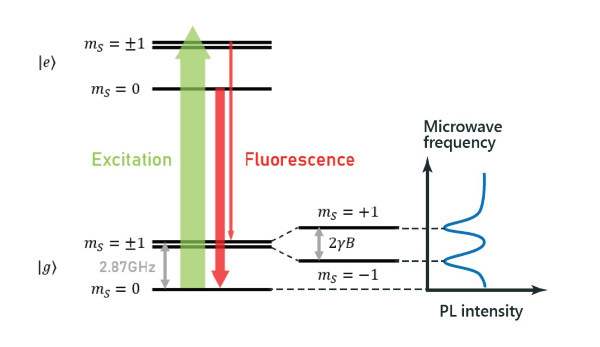
\includegraphics[width=0.5\textwidth]{figures/NVlevelwithESR.png}
%     % 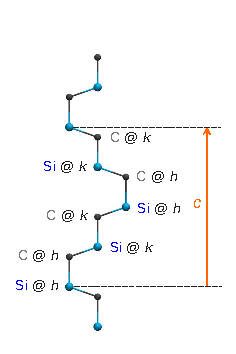
\includegraphics[width=0.38\textwidth]{figures/SiC-non-equiv-sites.pdf}%
%   \caption{Magnetometry with $\theta = 0$. Left shows the lifting of degeneracy of the spin system energy levels with the applied $\vec{B}$ field. Right shows the corresponding ODMR spectra and two EPR frequencies \cite{dnvweb}. \td{better caption}}%
% \label{fig:spin1_magnetometry}
% \end{wrapfigure}

\begin{figure}[h]
	\begin{center}
		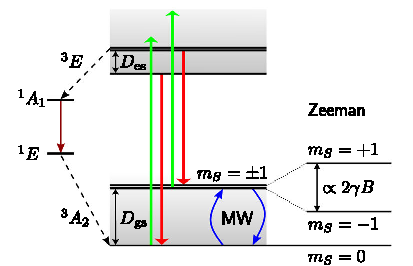
\includegraphics[width=0.7\textwidth]{figures/DNV-ODMR.pdf}
		% \missingfigure{Two panel figure. Panel 1 - energy level splitting of S=1 system being prop to gyromagnetic ratio. Panel 2 - ODMR Spectra} 
	\end{center}
	\caption{ODMR Magnetometry with $\theta = 0$. Degeneracy of the spin system energy levels is lifted with the applied $\vec{B}$ field \cite{Strner2021}. }
	\label{fig:spin1_magnetometry}
\end{figure}
%

\subsubsection{$\vec{B}$ at Angle $\theta$ to Defect Axis}
The Zeeman effect is proportional to $\cos\theta$, thus, when $\vec{B}$ is perpendicular to the defect axis the Zeeman effect reduces to zero, varying the azimuthal angle $\theta$ is effectively the same as scaling $B_0$ by $\cos \theta$.

\td{Reference how this reduction to zero can be exploited in electometry?}

\begin{figure}[h]
	\begin{center}
		% /        \missingfigure{ODMR or Energy Eigenvalues plot for $\theta = 0, 30, 60, 90$ showing the effective reduction of applied parallel field.}
		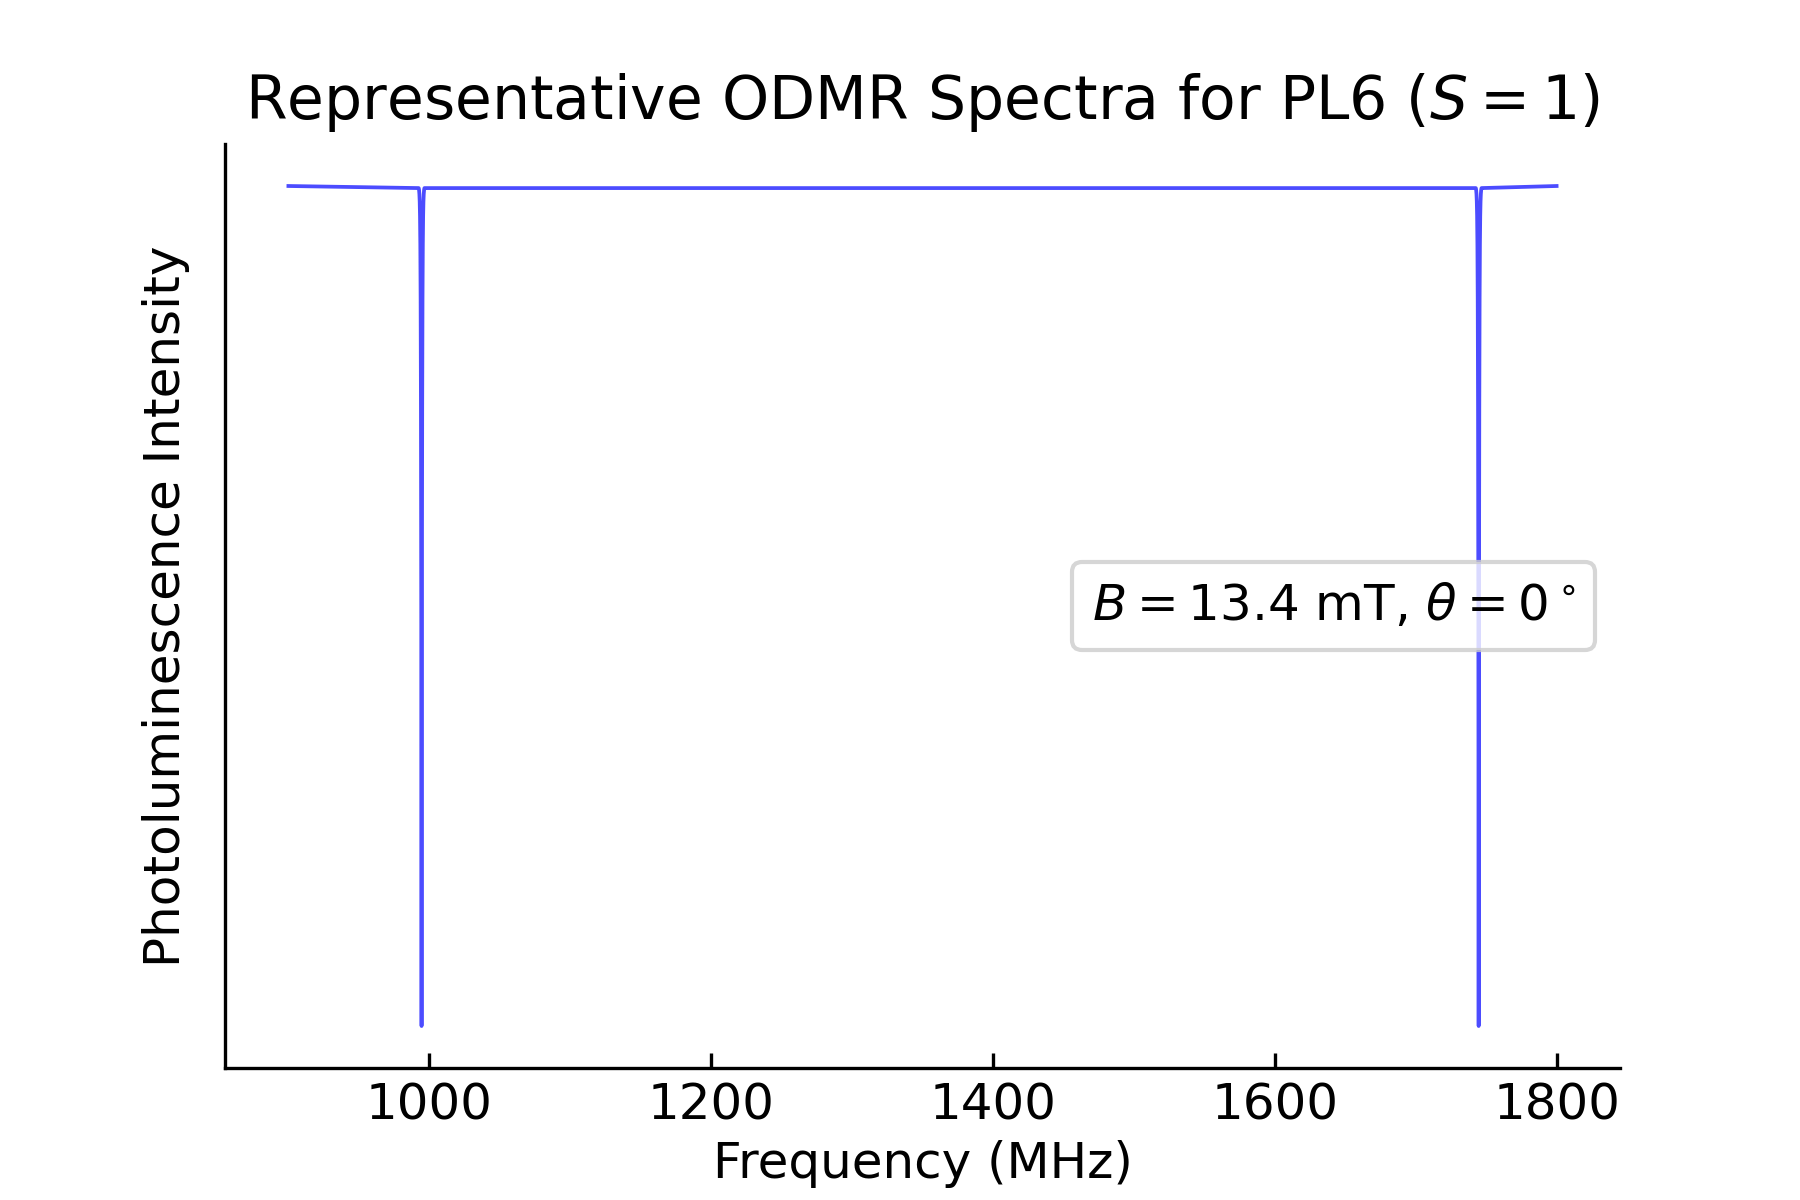
\includegraphics[width=\textwidth]{figures/PL6ODMRSpectra_theta_0_to_90.png}
	\end{center}
	\caption{ODMR/Energy level plot showing the reduction of the effective parallel $\vec{B}$ field with increasing $\theta$.}
	\label{fig:}
\end{figure}


\subsection{$S=1$ Vector Magnetometry}
Vector magnetometry with a $S=1$ system can be achieved by comparing the relative intensities from defects known to be at specific angles.

For example, in diamond the nitrogen vacancy is aligned with the tetragonal crystal structure and thus may take one of four orientations as illustrated in Figure \ref{fig:dnv_orientations}.

\begin{figure}[h]
	\begin{center}
		% \missingfigure{Sketch of DNV and possible defect orientations.}
		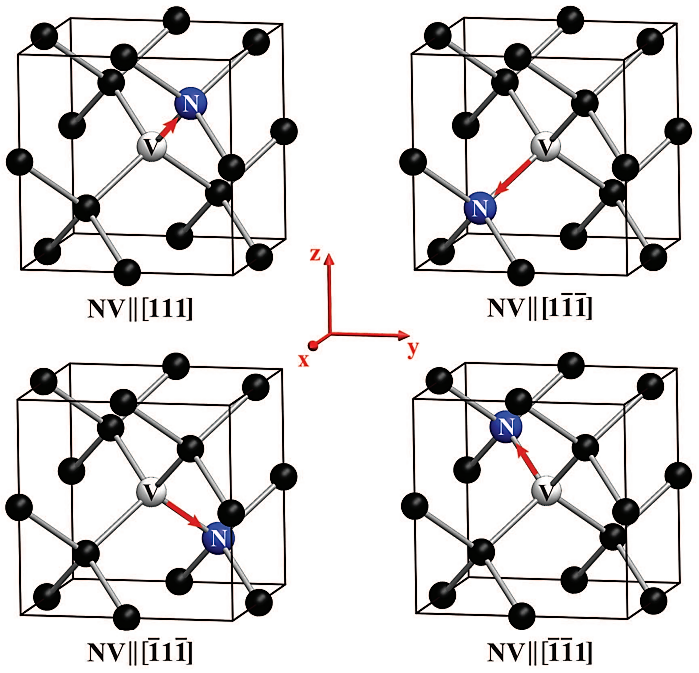
\includegraphics[width=0.45\textwidth]{figures/four_possible_NV_orientations.png}
	\end{center}
	\caption{Diagram showing the four possible orientations of NV centers in diamond \cite{pham}.}\label{fig:dnv_orientations}
\end{figure}


The 4 possible DNV orientations in the lattice are $111$, $1\overline{11}$, $\overline{1}1\overline{1}$ and $\overline{11}1$.
Once the projections of the magnetic field along these axes have been measures, we reconstruct the magnetic field in the laboratory frame.

The ODMR sprectrum for a sample of diamond with approximately equal distribution of the four defect orientations.

% # file:///home/conner/Downloads/e2015-60080-1.pdf
\td{Finish typing - link in comments}
The measured field components $m_i$ do not directly give the magnetic field $B_i$, but are affected by some noise in-
herent to the measurement which is accounted for using a maximum-likelihood method.

% The direction of $\vec{B}$ relative to the crystal lattice can then be determined by solving 
% \begin{equation}
%     \underbrace{
%     \frac{1}{\sqrt{3}}
%     \begin{pmatrix}        
%         1 & 1 & 1 \\ 
%         -1 & -1 & 1 \\ 
%         -1 & 1 & -1 \\ 
%         1 & -1 & -1 
% \end{pmatrix}}_{N}
%     \mathbf{\hat{B}} = 
%     \underbrace{
%     \begin{pmatrix}
%         \cos\theta_1 \\
%         \cos\theta_2 \\
%         \cos\theta_3 \\
%         \cos\theta_4 \\
%     \end{pmatrix}
% }_{\mathbf{c}}
%     \label{eq:}
% \end{equation}
% For which a solution may be determined 
% \begin{equation}
%     \mathbf{\hat{B}} = \left(N^T N\right)^{-1} N^T \mathbf{c}.   
%     \label{eq:}
% \end{equation}
%
% With knowledge of .. \td{Need to finish writing about knowing the miller index family of crystal can convert miller vector to lab vector}. 
%

\cite{Balasubramanian2008}
\td{Need to also look at this method and type up}

% \begin{tcolorbox}[colback=ediblue!5!white,colframe=ediblue!75!black,title={$S=1$ Magnetometry Summary}]
% \end{tcolorbox}

% \begin{summary}{%
% 		\subsection{$S=1$ Magnetometry Summary}%
% 		\label{spin1_magnetometry}%
%         \vspace{-0.5em}
% 	}%
%
% 	We may achieve vector magnetometry using a triplet state if
% \end{summary}

\begin{summary}{$S=1$ Magnetometry Summary}{sum:spin1magnet}

	We may achieve vector magnetometry using a triplet state if
	\begin{enumerate}
		\item We can identify three lines.
		\item We can use this equation which we have already written and we link:
		      \begin{equation}
                  \tcbhighmath{B_0 = \frac{f_1 - f_2}{2 \gamma}}
			      \tag{\ref{eq:s1_parallel_magnetometry}}
		      \end{equation}
	\end{enumerate}


\end{summary}
